\section{Interpolación mediante Funciones Splines}\label{sec:Rel3.2}

\begin{ejercicio} Determine $a, b$ y $c$ para que la siguiente función sea un spline cúbico:
\begin{equation*}
    s(x)=\left\{\begin{array}{lc}
        x^3 & 0\leq x \leq 1 \\
        \frac{1}{2}(x-1)^3 +a(x-1)^2 + b(x-1) + c& 1\leq x \leq 3 
    \end{array}\right.
\end{equation*}

Hemos de comprobar que $s\in {C}^{2}[0,3]$.

Para que $s$ sea continua, es necesario que:
\begin{equation*}
    \lim_{x\to1^-}s(x) = \lim_{x\to1^+}s(x) \Longrightarrow 1 = c
\end{equation*}

Para que $s\in \cc{C}^1[a,b]$, es necesario que $s'(x)$ sea continua:
\begin{equation*}
    s'(x)=\left\{\begin{array}{lc}
        3x^2 & 0\leq x \leq 1 \\
        \frac{3}{2}(x-1)^2 +2a(x-1) + b& 1\leq x \leq 3 
    \end{array}\right.
\end{equation*}
\begin{equation*}
    \lim_{x\to1^-}s'(x) = \lim_{x\to1^+}s'(x) \Longrightarrow 3 = b
\end{equation*}

Para que $s\in \cc{C}^2[a,b]$, es necesario que $s''(x)$ sea continua:
\begin{equation*}
    s''(x)=\left\{\begin{array}{lc}
        6x & 0\leq x \leq 1 \\
        3(x-1) +2a& 1\leq x \leq 3 
    \end{array}\right.
\end{equation*}
\begin{equation*}
    \lim_{x\to1^-}s'('x) = \lim_{x\to1^+}s''(x) \Longrightarrow 6=2a \Longrightarrow a=3
\end{equation*}

Por tanto, el spline cúbico es:
\begin{equation*}
    s(x)=\left\{\begin{array}{lc}
        x^3 & 0\leq x \leq 1 \\
        \frac{1}{2}(x-1)^3 +3(x-1)^2 + 3(x-1) + 1& 1\leq x \leq 3 
    \end{array}\right.
\end{equation*}

\end{ejercicio}

\begin{ejercicio}
    Obtenga el spline lineal que interpola los siguientes datos:
    \begin{equation*}
        \begin{array}{c|cccccc}
            x & -1 & 0 & 1 & 2 & 3 & 4 \\ \hline
            f(x) & -2 & 0 & 2 & 3 & 2 & 4
        \end{array}
    \end{equation*}

    El spline lineal es una función continua que une los puntos con rectas. Por tanto,
    \begin{itemize}
        \item \underline{$[-1,0]$}: $p_0(x)=2x$
        \item \underline{$[0,1]$}: $p_1(x)=2x$
        \item \underline{$[1,2]$}: $p_2(x)=x+1$
        \item \underline{$[2,3]$}: $p_3(x)=-x+5$
        \item \underline{$[3,4]$}: $p_4(x)=2x-4$
    \end{itemize}

    Por tanto, tenemos que:
    \begin{equation*}
        s(x)=\left\{\begin{array}{lll}
            2x & \text{si} & x\in [-1,0] \\
            2x & \text{si} & x\in [0,1] \\
            x+1 & \text{si} & x\in [1,2] \\
            -x+5 & \text{si} & x\in [2,3] \\
            2x-4 & \text{si} & x\in [3,4] \\
        \end{array}\right.
    \end{equation*}
\end{ejercicio}

\begin{ejercicio}
    Halle, si es posible, $s\in S_2(-1, 0, 3, 4)$ tal que:
    \begin{equation*}
        -s(-1)=s(2)=s(4)=1,\qquad \qquad s(0)=s(3)=0
    \end{equation*}


    En primer lugar, interpolo mediante Newton en el intervalo $[0,3]$, ya que también tengo el valor en $x=2$. Por tanto,
    \begin{equation*}
        \begin{array}{c|ccc}
            &&\mathbf{[0,3]} \\ \\
            x_i & f(x_i) \\ \\
            0 & \textbf{0} \\
            && \mathbf{\frac{1}{2}} \\ 
            2 & 1 && \mathbf{-\frac{1}{2}}\\
            && -1\\
            3 & 0
        \end{array}
    \end{equation*}

    Por tanto, tengo que $p_1(x)=\frac{1}{2}x -\frac{1}{2}x(x-2)$. Por tanto,
    \begin{equation*}
        p_1'(0)=\frac{1}{2}+1=\frac{3}{2}
        \qquad \qquad
        p_1'(3)=\frac{1}{2}-3+1 = -\frac{3}{2}
    \end{equation*}

    Interpolamos ahora los otros dos intervalos mediante el método de Hermite:
    \begin{equation*}
        \begin{array}{c|ccc}
            &&\mathbf{[-1,0]} \\ \\
            x_i & f(x_i) \\ \\
            -1 & \textbf{-1} \\
            && \textbf{1} \\ 
            0 & 0 && \mathbf{\frac{1}{2}}\\
            && \frac{3}{2}\\
            0 & 0
        \end{array}
        \qquad \left\|\qquad
        \begin{array}{c|ccc}
            &&\mathbf{[3,4]} \\ \\
            x_i & f(x_i) \\ \\
            3 & \textbf{0} \\
            && \mathbf{-\frac{3}{2}} \\ 
            3 & 0 && \mathbf{\frac{5}{2}}\\
            && 1\\
            4 & 1
        \end{array}\right.
    \end{equation*}

    Por tanto, tenemos que:
    \begin{equation*}
        s(x)=\left\{\begin{array}{lll}
            -1+(x+1)+\frac{1}{2}x(x+1) & \text{si} & x\in [-1,0] \\
            \frac{1}{2}x-\frac{1}{2}x(x-2) & \text{si} & x\in [0,3] \\
            -\frac{3}{2}(x-3)+\frac{5}{2}(x-3)^2 & \text{si} & x\in [3,4]
        \end{array}\right.
    \end{equation*}
    
\end{ejercicio}

\begin{ejercicio}
    Calcule el spline cuadrático que interpola los siguientes datos:
    \begin{equation*}
        \begin{array}{c|ccccc}
            x & -1 & 0 & 1 & 2 & 4 \\ \hline
            f(x) & -2 & 0 & 2 & 3 & 4
        \end{array}
    \end{equation*}
    y tal que $s'(1) = 0$.

    Sea el spline el siguiente:
    \begin{equation*}
        s(x)=\left\{\begin{array}{ccl}
            p_0(x)\in \bb{P}_2 & \text{si} & x\in [-1, 0[ \\
            p_{1}(x)\in \bb{P}_2 & \text{si} & x\in [0,1[ \\
            p_{2}(x)\in \bb{P}_2 & \text{si} & x\in [1,2[ \\
            p_{3}(x)\in \bb{P}_2 & \text{si} & x\in [2,4]
        \end{array} \right.
    \end{equation*}

    Interpolo cada uno de los intervalos. Empiezo en los intervalos $[0,1[$ y $[1,2[$, ya que tengo el valor de $s'(1)$.
    \begin{equation*}
        \begin{array}{c|ccc}
            &&\mathbf{[0,1[} \\ \\
            x_i & f(x_i) \\ \\
            0 & \textbf{0} \\
            && \textbf{2} \\ 
            1 & 2 && \textbf{-2}\\
            && 0\\
            1 & 2
        \end{array}
        \qquad \left\|\qquad
        \begin{array}{c|ccc}
            &&\mathbf{[1,2[} \\ \\
            x_i & f(x_i) \\ \\
            1 & \textbf{2} \\
            && \textbf{0} \\ 
            1 & 2 && \textbf{1}\\
            && 1\\
            2 & 3
        \end{array}\right.
    \end{equation*}
    Por tanto,
    \begin{equation*}
        p_1(x)=2x -2x(x-1) \qquad p_2(x)=2 +(x-1)^2
    \end{equation*}
    Como $s\in C^{1}[-1, 4]$,
    \begin{equation*}
        p_0'(0)=p_1'(0)=2-2(0-1)-0 = 4 \qquad 
        p_2'(2)=p_3'(2)=2(2-1) = 2
    \end{equation*}

    Sabiendo el valor de las derivadas, interpolo ahora mediante Hermite los dos polinomios que faltan.
    \begin{equation*}
        \begin{array}{c|ccc}
            &&\mathbf{[-1,0[} \\ \\
            x_i & f(x_i) \\ \\
            -1 & \textbf{-2} \\
            && \textbf{2} \\ 
            0 & 0 && \textbf{2}\\
            && 4\\
            0 & 0
        \end{array}
        \qquad \left\|\qquad
        \begin{array}{c|ccc}
            &&\mathbf{[2,4]} \\ \\
            x_i & f(x_i) \\ \\
            2 & \textbf{3} \\
            && \textbf{2} \\ 
            2 & 3 && \mathbf{-\frac{3}{4}}\\
            && \frac{1}{2}\\
            4 & 4
        \end{array}\right.
    \end{equation*}
    Por tanto,
    \begin{equation*}
        p_0(x)=-2+2(x+1)+2x(x+1) \qquad p_3(x)=3+2(x-2) -\frac{3}{4}(x-2)^2
    \end{equation*}

    En conclusión, tenemos que el spline pedido es:
    \begin{equation*}
        s(x)=\left\{\begin{array}{lll}
            p_0(x)=-2+2(x+1)+2x(x+1) & \text{si} & x\in [-1, 0[ \\
            p_1(x)=2x -2x(x-1) & \text{si} & x\in [0,1[ \\
            p_2(x)=2 +(x-1)^2 & \text{si} & x\in [1,2[ \\
            p_3(x)=3+2(x-2) -\frac{3}{4}(x-2)^2 & \text{si} & x\in [2,4]
        \end{array} \right.
    \end{equation*}
\end{ejercicio}

\begin{ejercicio}
    Obtenga el spline cúbico $s(x)$ con nodos $-1, 0, 1$, que verifica:
    \begin{equation*}
        s''(-1)=s''(1)=s(-1)=s(1)=0,\qquad \qquad s(0)=1
    \end{equation*}

    Tenemos que se trata de la interpolación de un spline cúbico natural. Resolvemos, por tanto, el sistema correspondiente.
    \begin{equation*}
        h_0=h_1 = 1 \qquad \Delta_0 = -\Delta_1= 1
    \end{equation*}

    El sistema, por tanto, a resolver es:
    \begin{equation*}
        \left(\begin{array}{ccc}
            2 & 1 & 0 \\
            1 & 4 & 1 \\
            0 & 1 & 2
        \end{array}\right)
        \left(\begin{array}{c}
            s'(-1) \\ s'(0) \\ s'(1)
        \end{array}\right)
        = 3 \left(\begin{array}{c}
            1 \\ 0 \\ -1
        \end{array}\right) \Longrightarrow \left\{\begin{array}{c}
            s'(-1)=-s'(1)=\frac{3}{2} \\
            s'(0)=0
        \end{array}\right.
    \end{equation*}


    Interpolamos mediante Hermite en cada intervalo:
    \begin{equation*}
        \begin{array}{c|cccc}
            &&\mathbf{[-1, 0]} \\ \\
            x_i & f(x_i) \\ \\
            -1 & \textbf{0} \\
            && \mathbf{\frac{3}{2}}\\
            -1 & 0 && \mathbf{-\frac{1}{2}}\\
            && 1 && \mathbf{-\frac{1}{2}}\\ 
            0 & 1 && -1\\
            && 0\\
            0 & 1
        \end{array}
        \quad \left\|\quad
        \begin{array}{c|cccc}
            &&\mathbf{[0,1]} \\ \\
            x_i & f(x_i) \\ \\
            0 & \textbf{1} \\
            && \mathbf{0}\\
            0 & 1 && \mathbf{-1}\\
            && -1 && \mathbf{\frac{1}{2}}\\ 
            1 & 0 && -\frac{1}{2}\\
            && -\frac{3}{2}\\
            1 & 0
        \end{array}\right.
    \end{equation*}

    Por tanto, el spline queda:
    \begin{equation*}
        s(x)=\left\{\begin{array}{ccl}
            \frac{3}{2}(x+1)-\frac{1}{2}(x+1)^2-\frac{1}{2}x(x+1)^2 & \text{si} & x\in [-1, 0] \\
            1-x^2+\frac{1}{2}(x-1)x^2 & \text{si} & x\in [0,1]
        \end{array} \right.
    \end{equation*}
\end{ejercicio}

\begin{ejercicio}
    Calcule el spline cúbico $s(x) \in S_3(1, 2, 3, 4)$ natural que interpola los siguientes datos:
    \begin{equation*}
        s(1) = 1,\qquad s(2) = 2,\qquad s(3) = -1,\qquad s(4) = 3.
    \end{equation*}



    Sea el spline el siguiente:
    \begin{equation*}
        s(x)=\left\{\begin{array}{ccl}
            p_0(x)\in \bb{P}_3 & \text{si} & x\in [1, 2] \\
            p_{1}(x)\in \bb{P}_3 & \text{si} & x\in [2, 3] \\
            p_{2}(x)\in \bb{P}_3 & \text{si} & x\in [3, 4] \\
        \end{array} \right.
    \end{equation*}

    Aplicamos el sistema que se ha visto en clase para calcular los splines cúbicos. Tenemos que:
    \begin{equation*}
        h_n = x_{n+1} - x_n \qquad h_0=h_1 = h_2 = 1
    \end{equation*}
    \begin{equation*}
        \Delta_n = \frac{s(x_{n+1}) - s(x_n)}{h_n} \qquad \Delta_0=1 \quad \Delta_1=-3 \quad \Delta_2=4
    \end{equation*}

    Sean las incógnitas del sistema $d_i = s'(x_i)$. El sistema a resolver es:
    \begin{equation*}
        \left(\begin{array}{cccc}
            2 & 1 & 0 & 0\\
            1 & 4 & 1 & 0\\
            0 & 1 & 4 & 1 \\
            0 & 0 & 1 & 2
        \end{array}\right)
        \left(\begin{array}{ccc}
            d_0 \\ d_1 \\ d_2 \\ d_3
        \end{array}\right) =
        3\left(\begin{array}{ccc}
            1 \\ -2 \\ 1 \\ 4
        \end{array}\right) \Longrightarrow \left\{\begin{array}{l}
            d_0=s'(x_0)=\frac{38}{15} \\ d_1=s'(x_1)=-\frac{31}{15} \\ d_2=s'(x_2) = -\frac{4}{15} \\ d_3=s'(x_3) = \frac{92}{15}
        \end{array}\right.
    \end{equation*}

    Interpolamos mediante Hermite en cada intervalo:
    \begin{equation*}
        \begin{array}{c|cccc}
            &&\mathbf{[1,2]} \\ \\
            x_i & f(x_i) \\ \\
            1 & \textbf{1} \\
            && \mathbf{\frac{38}{15}}\\
            1 & 1 && \mathbf{-\frac{23}{15}}\\
            && 1 && -\mathbf{\frac{23}{15}}\\ 
            2 & 2 && -\frac{46}{15}\\
            && -\frac{31}{15}\\
            2 & 2
        \end{array}
        \quad \left\|\quad
        \begin{array}{c|cccc}
            &&\mathbf{[2,3]} \\ \\
            x_i & f(x_i) \\ \\
            2 & \textbf{2} \\
            && \mathbf{-\frac{31}{15}}\\
            2 & 2 && \mathbf{-\frac{14}{15}}\\
            && -3 && \mathbf{\frac{11}{3}}\\ 
            3 & -1 && \frac{41}{15}\\
            && -\frac{4}{15}\\
            3 & -1
        \end{array}\right.
        \quad \left\|\quad
        \begin{array}{c|cccc}
            &&\mathbf{[3, 4]} \\ \\
            x_i & f(x_i) \\ \\
            3 & \textbf{-1} \\
            && \mathbf{-\frac{4}{15}}\\
            3 & -1 && \mathbf{\frac{64}{15}}\\
            && 4 && \mathbf{-\frac{32}{15}}\\ 
            4 & 3 && \frac{32}{15}\\
            && \frac{92}{15}\\
            4 & 3
        \end{array}\right.
    \end{equation*}

    Por tanto, el spline queda:
    \begin{equation*}
        s(x)=\left\{\begin{array}{ccl}
            1+\frac{38}{15}(x-1)-\frac{23}{15}(x-1)^2 -\frac{23}{15}(x-1)^2(x-2)& \text{si} & x\in [1, 2] \\
            2-\frac{31}{14}(x-2)-\frac{14}{15}(x-2)^2 +\frac{11}{3}(x-2)^2(x-3) & \text{si} & x\in [2, 3] \\
            -1-\frac{4}{15}(x-3)+\frac{64}{15}(x-3)^2 - \frac{32}{15}(x-3)^2(x-4)& \text{si} & x\in [3, 4] \\
        \end{array} \right.
    \end{equation*}
\end{ejercicio}

\begin{ejercicio}
    Calcule el spline cúbico $s(x) \in S_3(1, 2, 3, 4)$ periódico que interpola los siguientes datos:
    \begin{equation*}
        s(1) = 1,\qquad s(2) = 2,\qquad s(3) = -1,\qquad s(4) = 1.
    \end{equation*}

    Sea el spline el siguiente:
    \begin{equation*}
        s(x)=\left\{\begin{array}{ccl}
            p_0(x)\in \bb{P}_3 & \text{si} & x\in [1, 2] \\
            p_{1}(x)\in \bb{P}_3 & \text{si} & x\in [2, 3] \\
            p_{2}(x)\in \bb{P}_3 & \text{si} & x\in [3, 4] \\
        \end{array} \right.
    \end{equation*}

    Aplicamos el sistema que se ha visto en clase para calcular los splines cúbicos. Tenemos que:
    \begin{equation*}
        h_n = x_{n+1} - x_n \qquad h_0=h_1 = h_2 = 1
    \end{equation*}
    \begin{equation*}
        \Delta_n = \frac{s(x_{n+1}) - s(x_n)}{h_n} \qquad \Delta_0=1 \quad \Delta_1=-3 \quad \Delta_2=2
    \end{equation*}

    Sean las incógnitas del sistema $d_i = s'(x_i)$. El sistema a resolver, teniendo en cuenta que se trata de un spline periódico, es:
    \begin{equation*}
        \left(\begin{array}{cccc}
            1 & 0 & 0 & -1\\
            1 & 4 & 1 & 0\\
            0 & 1 & 4 & 1 \\
            2 & 1 & 1 & 2
        \end{array}\right)
        \left(\begin{array}{ccc}
            d_0 \\ d_1 \\ d_2 \\ d_3
        \end{array}\right) =
        3\left(\begin{array}{ccc}
            0 \\ -2 \\ -1 \\ 3
        \end{array}\right) \Longrightarrow \left\{\begin{array}{l}
            d_0=s'(x_0)=3 \\ d_1=s'(x_1)=-2 \\ d_2=s'(x_2) = -1 \\ d_3=s'(x_3) = 3
        \end{array}\right.
    \end{equation*}

    Interpolamos mediante Hermite en cada intervalo:
    \begin{equation*}
        \begin{array}{c|cccc}
            &&\mathbf{[1,2]} \\ \\
            x_i & f(x_i) \\ \\
            1 & \textbf{1} \\
            && \mathbf{3}\\
            1 & 1 && \mathbf{-2}\\
            && 1 && \mathbf{-1}\\ 
            2 & 2 && -3\\
            && -2\\
            2 & 2
        \end{array}
        \quad \left\|\quad
        \begin{array}{c|cccc}
            &&\mathbf{[2,3]} \\ \\
            x_i & f(x_i) \\ \\
            2 & \textbf{2} \\
            && \mathbf{-2}\\
            2 & 2 && \mathbf{-1}\\
            && -3 && \mathbf{3}\\ 
            3 & -1 && 2\\
            && -1\\
            3 & -1
        \end{array}\right.
        \quad \left\|\quad
        \begin{array}{c|cccc}
            &&\mathbf{[3, 4]} \\ \\
            x_i & f(x_i) \\ \\
            3 & \mathbf{-1} \\
            && \mathbf{-1}\\
            3 & -1 && \mathbf{3}\\
            && 2 && \mathbf{-2}\\ 
            4 & 1 && 1\\
            && 3\\
            4 & 1
        \end{array}\right.
    \end{equation*}

    Por tanto, el spline queda:
    \begin{equation*}
        s(x)=\left\{\begin{array}{ccl}
            1+3(x-1)-2(x-1)^2 -(x-1)^2(x-2)& \text{si} & x\in [1, 2] \\
            2-2(x-2)-(x-2)^2 +3(x-2)^2(x-3) & \text{si} & x\in [2, 3] \\
            -1-(x-3)+3(x-3)^2-2(x-3)^2(x-4) & \text{si} & x\in [3, 4] \\
        \end{array} \right.
    \end{equation*}
\end{ejercicio}

\begin{ejercicio}
    Obtenga el spline $s(x) \in S^1_3 (-1, 0, 2)\footnote{$S^1_3$ denota los spline cúbicos de clase 1.}$ que interpola:
    \begin{equation*}
        \begin{array}{ccc}
            s(-1)=-6 & s(0)=-3 & s(2)=33 \\
            s'(-1)=9 & s'(0)=0 & s'(2)=48 \\
        \end{array}
    \end{equation*}

    Interpolamos mediante Hermite en cada intervalo:
    \begin{equation*}
        \begin{array}{c|cccc}
            &&\mathbf{[-1, 0]} \\ \\
            x_i & f(x_i) \\ \\
            -1 & \mathbf{-6} \\
            && \mathbf{9}\\
            -1 & -6 && \mathbf{-6}\\
            && 3 && \mathbf{3}\\ 
            0 & -3 && -3\\
            && 0\\
            0 & -3
        \end{array}
        \quad \left\|\quad
        \begin{array}{c|cccc}
            &&\mathbf{[0,2]} \\ \\
            x_i & f(x_i) \\ \\
            0 & \mathbf{-3} \\
            && \mathbf{0}\\
            0 & -3 && \mathbf{9}\\
            && 18 && \mathbf{3}\\ 
            2 & 33 && 15\\
            && 48\\
            2 & 33
        \end{array}\right.
    \end{equation*}

    Por tanto, el spline queda:
    \begin{equation*}
        s(x)=\left\{\begin{array}{lll}
            -6+9(x+1)-6(x+1)^2 +3(x+1)^2x & \text{si} & x\in [-1, 0] \\
            -3 +9x^2+3x^2(x-2) & \text{si} & x\in [0, 2] \\
        \end{array} \right.
    \end{equation*}
    
\end{ejercicio}

\begin{ejercicio}
    Deduzca el spline cúbico $s(x) \in S_3(-1,0,1,3)$ que interpola los siguientes datos:
    \begin{equation*}
        s(-1) = -2,\quad s'(-1) = 2,\quad s(0) = 0,\quad s'(0) = 0,\quad s(1) = 2,\quad s(3) = 30.
    \end{equation*}

    Como el spline es cúbico y hay 4 nodos, sea el spline el siguiente:
    \begin{equation*}
        s(x)=\left\{\begin{array}{ccl}
            p_0(x)\in \bb{P}_3 & \text{si} & x\in [-1, 0] \\
            p_{1}(x)\in \bb{P}_3 & \text{si} & x\in [0,1] \\
            p_{2}(x)\in \bb{P}_3 & \text{si} & x\in [1,3] \\
        \end{array} \right.
    \end{equation*}

    Como en este caso no dan información sobre el tipo del spline calculado, aplicamos el método general mediante Hermite. Ya que tenemos el valor de $s'(-1)$ y de $s'(0)$, trabajamos en el intervalo $[-1,0]$:
    \begin{equation*}
        \begin{array}{c|cccc}
            &&\mathbf{[-1, 0]} \\ \\
            x_i & f(x_i) \\ \\
            -1 & \mathbf{-2} \\
            && \mathbf{2}\\
            -1 & -2 && \mathbf{0}\\
            && 2 && \mathbf{-2}\\ 
            0 & 0 && -2\\
            && 0\\
            0 & 0
        \end{array}
    \end{equation*}

    Por tanto, tengo que $p_0(x)=-2+2(x+1)-2x(x+1)^2$.
    \begin{equation*}
        p'_0(x)=2-2(x+1)^2-4x(x+1)
        \qquad
        p''_0(x)=-4(x+1)-4(x+1)-4x = -12x-8
    \end{equation*}

    Para interpolar en el intervalo $[0,1]$, hago uso del resultado teórico de que:
    \begin{equation*}
        f[\overbrace{x_0,\dots,x_0}^{k+1}] = \frac{f^{(k)}(x_0)}{k!}
    \end{equation*}
    
    Por tanto:
    \begin{equation*}
        s[0,0]=s'(0)=0
        \qquad
        s[0,0,0]=\frac{s''(0)}{2}=\frac{-8}{2}=-4
    \end{equation*}
    \begin{equation*}
        \begin{array}{c|cccc}
            &&\mathbf{[0,1]} \\ \\
            x_i & f(x_i) \\ \\
            0 & \mathbf{0} \\
            && \mathbf{0}\\
            0 & 0 && \mathbf{-4}\\
            && 0 && \mathbf{6}\\ 
            0 & 0 && 2\\
            && 2\\
            1 & 2
        \end{array}
    \end{equation*}
    Por tanto, tengo que $p_1(x)=-4x^2+6x^3$.
    \begin{equation*}
        p'_1(x)=-8x+18x^2
        \qquad
        p''_1(x)=-8+36x
    \end{equation*}

    Para interpolar en el intervalo $[1,3]$, uso que:
    \begin{equation*}
        s[1,1]=s'(1)=10
        \qquad
        s[1,1,1]=\frac{s''(1)}{2}=\frac{28}{2}=14
    \end{equation*}
    \begin{equation*}
        \begin{array}{c|cccc}
            &&\mathbf{[1,3]} \\ \\
            x_i & f(x_i) \\ \\
            1 & \mathbf{2} \\
            && \mathbf{10}\\
            1 & 2 && \mathbf{14}\\
            && 10 && \mathbf{-6}\\ 
            1 & 2 && 2\\
            && 14\\
            3 & 30
        \end{array}
    \end{equation*}
    Por tanto, tengo que $p_2(x)=2+10(x-1)+10(x-1)^2-6(x-1)^3$.


    Por tanto, tenemos que el spline queda:
    \begin{equation*}
        s(x)=\left\{\begin{array}{lll}
            p_0(x)=-2+2(x+1)-2x(x+1)^2 & \text{si} & x\in [-1, 0] \\
            p_1(x)=-4x^2+6x^3 & \text{si} & x\in [0,1] \\
            p_2(x)=2+10(x-1)+14(x-1)^2-6(x-1)^3 & \text{si} & x\in [1,3] \\
        \end{array} \right.
    \end{equation*}

    
\end{ejercicio}

\begin{ejercicio}
    Calcule la expresión del spline cúbico de clase uno que interpola los siguientes datos.
    \begin{equation*}
        \begin{array}{c|cccc}
            x_i & -1 & 0 & 1 & 2 \\ \hline
            f_i & 0 & 0 & 1 & 1 \\ \hline
            f_i' & 0 & 0 & 0 & 0\\
        \end{array}
    \end{equation*}

    Dibuje su gráfica.

    En primer lugar, interpolamos mediante Hermite en cada intervalo:
    \begin{equation*}
        \begin{array}{c|cccc}
            &&\mathbf{[-1, 0]} \\ \\
            x_i & f(x_i) \\ \\
            -1 & \mathbf{0} \\
            && \mathbf{0}\\
            -1 & 0 && \mathbf{0}\\
            && 0 && \mathbf{0}\\ 
            0 & 0 && 0\\
            && 0\\
            0 & 0
        \end{array}
        \quad \left\|\quad
        \begin{array}{c|cccc}
            &&\mathbf{[0,1]} \\ \\
            x_i & f(x_i) \\ \\
            0 & \mathbf{0} \\
            && \mathbf{0}\\
            0 & 0 && \mathbf{1}\\
            && 1 && \mathbf{-2}\\ 
            1 & 1 && -1\\
            && 0\\
            1 & 1
        \end{array}\right.
        \quad \left\|\quad
        \begin{array}{c|cccc}
            &&\mathbf{[1,2]} \\ \\
            x_i & f(x_i) \\ \\
            1 & \mathbf{1} \\
            && \mathbf{0}\\
            1 & 1 && \mathbf{0}\\
            && 0 && \mathbf{0}\\ 
            2 & 1 && 0\\
            && 0\\
            2 & 1
        \end{array}\right.
    \end{equation*}

    Por tanto, tenemos que el spline queda:
    \begin{equation*}
        s(x)=\left\{\begin{array}{lll}
            p_0(x)=0 & \text{si} & x\in [-1, 0] \\
            p_1(x)=x^2-2x^2(x-1) & \text{si} & x\in [0,1] \\
            p_2(x)=1 & \text{si} & x\in [1,3] \\
        \end{array} \right.
    \end{equation*}

    Dibujo ahora la función, donde el intervalo $[0,1]$ es así ya que sé que el spline es de clase 1.

    \begin{figure}[H]
        \centering
        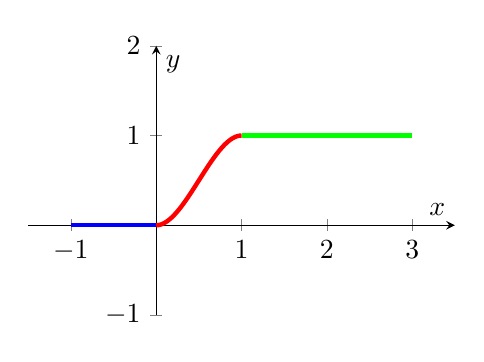
\begin{tikzpicture}
        \begin{axis}[
            xlabel=$x$,
            ylabel=$y$,
            xmin=-1.5,
            xmax=3.5,
            ymin=-1,
            ymax=2,
            axis lines=middle,
            width=7cm,
            height=5cm,
            samples=90 % número de muestras para la función
        ]
        
        \addplot[blue, ultra thick,domain=-1:0] {0};
        \addplot[red, ultra thick,domain=0:1] {3*x^2-2*x^3};
        \addplot[green, ultra thick,domain=1:3] {1};
            
        \end{axis}
        \end{tikzpicture}
    \end{figure}
\end{ejercicio}

\begin{ejercicio}
    Halla el spline cúbico $s(x)$ de extremo sujeto que interpola los datos $s(0) = 8,\;s(2) =0,\;$ $s(4) = 8$ y satisface las dos condiciones adicionales $s'(0)=~-~12, \;s'(4) = 12$.

    Resolvemos empleando el sistema visto en clase.
    \begin{equation*}
        h_0=h_1=2 \qquad \Delta_0=\frac{0-8}{2}=-4 \qquad \Delta_1=\frac{8-0}{2}=4
    \end{equation*}
    
    Teniendo en cuenta que se trata de un spline ligado, tenemos que el sistema queda:
    \begin{equation*}
        \left(\begin{array}{ccc}
            1 & 0 & 0 \\
            \frac{1}{2} & 2 & \frac{1}{2} \\
            0 & 0 & 1
        \end{array}\right)
        \left(\begin{array}{c}
            s'(0) \\ s'(2) \\ s'(4)
        \end{array}\right)
        = \left(\begin{array}{c}
            -12 \\ 0 \\ 12
        \end{array}\right) \Longrightarrow \left\{\begin{array}{l}
            s'(0)=-12 \\
            s'(2)=0 \\
            s'(4)=12
        \end{array}\right.
    \end{equation*}

    Interpolamos mediante Hermite en cada intervalo:
    \begin{equation*}
        \begin{array}{c|cccc}
            &&\mathbf{[0,2]} \\ \\
            x_i & f(x_i) \\ \\
            0 & \mathbf{8} \\
            && \mathbf{-12}\\
            0 & 8 && \mathbf{4}\\
            && -4 && \mathbf{-1}\\ 
            2 & 0 && 2\\
            && 0\\
            2 & 0
        \end{array}
        \quad \left\|\quad
        \begin{array}{c|cccc}
            &&\mathbf{[2,4]} \\ \\
            x_i & f(x_i) \\ \\
            2 & \mathbf{0} \\
            && \mathbf{0}\\
            2 & 0 && \mathbf{2}\\
            && 4 && \mathbf{1}\\ 
            4 & 8 && 4\\
            && 12\\
            4 & 8
        \end{array}\right.
    \end{equation*}

    Por tanto, el spline queda:
    \begin{equation*}
        s(x)=\left\{\begin{array}{lll}
            8-12x +4x^2 -x^2(x-2) & \text{si} & x\in [0,2] \\
            2(x-2)^2 +(x-2)^2(x-4) & \text{si} & x\in [2,4] \\
        \end{array} \right.
    \end{equation*}

    
\end{ejercicio}

\begin{ejercicio}
    Justifique la veracidad o falsedad de la siguiente afirmación:

    ``Todo polinomio de grado menor o igual que tres es un spline cúbico natural para el conjunto de nodos $x_0 < x_1 < \dots < x_n$''.\\

    Sea el polinomio $p(x)=x^3\in \bb{P}_3[x]$. Tenemos que:
    \begin{equation*}
        p'(x)=3x^2 \qquad p''(x)=6x
    \end{equation*}

    Por tanto, como $p''(x)=0 \Longleftrightarrow x=0$, tenemos que no es posible que sea un spline natural ya que $$p''(a)=p''(b)=0 \Longleftrightarrow a=b=0$$

    No obstante, tenemos que $a\neq b$, por lo que llegamos a una contradicción y tenemos que $p(x)=x^3$ no es un spline natural, por lo que el enunciado es \textbf{falso}.

    No obstante, sí sabemos que todo $p\in \bb{P}_n$ es un spline de grado $n$.
\end{ejercicio}

\begin{ejercicio}
    ¿Cuál es el spline cúbico que interpola los datos
    \begin{equation*}
        \begin{array}{c|cccc}
            x_i & -2 & -1 & 1 & 2 \\ \hline
            f_i & 2 & 1 & 5 & 10
        \end{array}
    \end{equation*}
    y satisface las condiciones adicionales $s(0) = s'(0) = 2$? Justifique su respuesta.

    Como el spline es cúbico y hay 4 nodos, sea el spline el siguiente:
    \begin{equation*}
        s(x)=\left\{\begin{array}{ccl}
            p_0(x)\in \bb{P}_3 & \text{si} & x\in [-2, -1] \\
            p_{1}(x)\in \bb{P}_3 & \text{si} & x\in [-1, 1] \\
            p_{2}(x)\in \bb{P}_3 & \text{si} & x\in [1,2] \\
        \end{array} \right.
    \end{equation*}

    Ya que las condiciones adicionales están en el intervalo $[-1, 1]$, interpolo en dicho intervalo en primer lugar.
    \begin{equation*}
        \begin{array}{c|cccc}
            &&\mathbf{[-1,1]} \\ \\
            x_i & f(x_i) \\ \\
            -1 & \mathbf{1} \\
            && \mathbf{1}\\
            0 & 2 && \mathbf{1}\\
            && 2 && \mathbf{0}\\ 
            0 & 2 && 1\\
            && 3\\
            1 & 5
        \end{array}
    \end{equation*}

    Por tanto,
    \begin{equation*}
        p_1(x)=1+(x+1)+x(x+1)=2+2x+x^2
    \end{equation*}
    \begin{equation*}
    p_1'(x)=2+2x
    \qquad
    p_1''(x)=2
    \end{equation*}

    Por tanto, como $s\in \cc{C}^2[-2,2]$, tengo que:
    \begin{equation*}
        s'(-1)=0 \qquad s'(1)=4 \qquad s''(-1)=2 \qquad s''(1)=2
    \end{equation*}

    Tenemos el resultado teórico de que:
    \begin{equation*}
        f[\overbrace{x_0,\dots,x_0}^{k+1}] = \frac{f^{(k)}(x_0)}{k!}
    \end{equation*}

    Por tanto,
    \begin{equation*}
        s[-1,-1,-1]=1 \qquad s[1,1,1]=1
    \end{equation*}
    
    interpolo mediante Hermite en los otros intervalos:
    \begin{equation*}
        \begin{array}{c|cccc}
            &&\mathbf{[-2, -1]} \\ \\
            x_i & f(x_i) \\ \\
            -2 & \mathbf{2} \\
            && \mathbf{-1}\\
            -1 & 1 && \mathbf{1}\\
            && 0 && \mathbf{0}\\ 
            -1 & 1 && 1\\
            && 0\\
            -1 & 1
        \end{array}
        \qquad \left\|\qquad
        \begin{array}{c|cccc}
            &&\mathbf{[1, 2]} \\ \\
            x_i & f(x_i) \\ \\
            1 & \mathbf{5} \\
            && \mathbf{4}\\
            1 & 5 && \mathbf{1}\\
            && 4 && \mathbf{0}\\ 
            1 & 5 && 1\\
            && 5\\
            2 & 10
        \end{array}\right.
    \end{equation*}


    Por tanto, el spline pedido es:
    \begin{equation*}
        s(x)=\left\{\begin{array}{lll}
            p_0(x)=2-(x+1)+(x+2)(x+1) & \text{si} & x\in [-2, -1] \\
            p_1(x)=1+2x+x^2 & \text{si} & x\in [-1, 1] \\
            p_{2}(x)=5+4(x-1)+(x-1)^2 & \text{si} & x\in [1,2] \\
        \end{array} \right.
    \end{equation*}

    De hecho, tenemos que $s(x)=(x+1)^2+1 \qquad \forall x\in [-2,2]$.
\end{ejercicio}

\begin{ejercicio}
    Para cierta función $f: [-2, 1] \to \bb{R}$ se obtiene la tabla de datos
    \begin{equation*}
        \begin{array}{c|ccc}
            x_i & -2 & -1 & 1 \\ \hline
            f_i & 4 & 3 & 5
        \end{array}
    \end{equation*}

    \begin{enumerate}
        \item Calcule el spline cuadrático $s(x)$ que interpola tales datos y, además, satisface la condición $s(0) = 3$.

        Sea el spline:
        \begin{equation*}
            s(x)=\left\{\begin{array}{lll}
                p_0(x)\in \bb{P}_2 & \text{si} & x\in [-2, -1]\\
                p_1(x)\in \bb{P}_2 & \text{si} & x\in [-1, 1]\\
            \end{array} \right.
        \end{equation*}

        Interpolamos en primer lugar en el intervalo $[-1,1]$, ya que se da la condición adicional de que $s(0)=3$.
        \begin{equation*}
            \begin{array}{c|ccc}
                &&\mathbf{[-1, 1]} \\ \\
                x_i & f(x_i) \\ \\
                -1 & \textbf{3} \\
                && \textbf{0} \\ 
                0 & 3 && \textbf{1}\\
                && 2\\
                1 & 5
            \end{array}
        \end{equation*}

        Por tanto, tenemos que $p_1(x)=3+x(x+1)=x^2+x+3$. Como $s\in C^1[-2,1]$, tenemos que $s'(-1)=-1$.
        \begin{equation*}
            \begin{array}{c|ccc}
                &&\mathbf{[-2, -1]} \\ \\
                x_i & f(x_i) \\ \\
                -2 & \textbf{4} \\
                && \textbf{-1} \\ 
                -1 & 3 && \textbf{0}\\
                && -1\\
                -1 & 3
            \end{array}
        \end{equation*}

        Por tanto, tenemos $p_0(x)=4-(x+2)=-x+2$. Por tanto,
        \begin{equation*}
            s(x)=\left\{\begin{array}{lll}
                -x+2 & \text{si} & x\in [-2, -1]\\
                x^2+x+3 & \text{si} & x\in [-1, 1]\\
            \end{array} \right.
        \end{equation*}

        \item A partir de lo obtenido en el apartado anterior, halle una aproximación de $\displaystyle \int_{-2}^0 f(x)dx$.
        \begin{multline*}
            \int_{-2}^0 f(x)dx \approx \int_{-2}^{-1} s(x)dx + \int_{-1}^0 s(x)dx = \left[-\frac{x^2}{2}+2x\right]^{-1}_{-2} + \left[\frac{x^3}{3}+\frac{x^2}{2}+3x\right]^{0}_{-1} 
            =\\=
            -\frac{1}{2}-2+\frac{4}{2}+4 +\frac{1}{3}-\frac{1}{2}+3 = \frac{19}{3}
        \end{multline*}
    \end{enumerate}
\end{ejercicio}

\begin{ejercicio}
    Se considera la función:
    \begin{equation*}
        s(x)=\left\{\begin{array}{lll}
            -3x^2 + 9x - 7 & \text{si} & x\in [-1, 1]\\
            p(x) & \text{si} & x\in [1, 3]\\
            -x^3 + 12x^2 - 42x + 46 & \text{si} & x\in [3, 5]\\
        \end{array} \right.
    \end{equation*}

    \begin{enumerate}
        \item Determine $p(x)$ para que $s(x)$ sea un spline cúbico de clase 2.

        Por el carácter local de la derivabilidad, y sabiendo que al ser $s\in \cc{C}^2[-1,5]$, tengo:
        \begin{equation*}
            s'(x)=\left\{\begin{array}{lll}
                -6x + 9 & \text{si} & x\in [-1, 1]\\
                p'(x) & \text{si} & x\in [1, 3]\\
                -3x^2 + 24x - 42 & \text{si} & x\in [3, 5]\\
            \end{array} \right.
        \end{equation*}
        \begin{equation*}
            s''(x)=\left\{\begin{array}{lll}
                -6 & \text{si} & x\in [-1, 1]\\
                p''(x) & \text{si} & x\in [1, 3]\\
                -6x + 24& \text{si} & x\in [3, 5]\\
            \end{array} \right.
        \end{equation*}

        Por tanto, tengo que:
        \begin{equation*}
            s(1)=-1 \qquad s(3)=1 \qquad s'(1)=3 \qquad s'(3)=3 \qquad s''(1)=-6 \qquad s''(3)=6
        \end{equation*}

        Cabe destacar que para calcular $p$ son solo necesarias 4 condiciones. Por tanto, elijo las 4 primeras.

        Por tanto, interpolando mediante Hermite:
        \begin{equation*}
            \begin{array}{c|cccc}
                &&\mathbf{[1,3]} \\ \\
                x_i & f(x_i) \\ \\
                1 & \mathbf{-1} \\
                && \mathbf{3}\\
                1 & -1 && \mathbf{-1}\\
                && 1 && \mathbf{1}\\ 
                3 & 1 && 1\\
                && 3\\
                3 & 1
            \end{array}
        \end{equation*}

        Por tanto,
        \begin{equation*}
            p(x)=-1+3(x-1)-(x-1)^2+(x-1)^2(x-3)
        \end{equation*}

        \item ¿Puede ser $s(x)$ un spline cúbico natural? Justifique tu respuesta.

        No, ya que si fuese natural tendría que cumplirse que $s''(-1)=s''(5)=0$. No obstante, $s''(-1)=-6.$

        \item ¿Cuánto valen $s'(0)$ y $s''(2)$?

        Tengo que $s'(0)=9$. Calculamos ahora $s''(2)=p''(2)$:
        \begin{equation*}
            p'(x)=3-2(x-1)+2(x-1)(x-3) +(x-1)^2
            \qquad
            p''(x)=-2+2(x-3)+2(x-1)+2(x-1)
        \end{equation*}

        Por tanto, $p''(2)=s''(2)=-2+2(-1)+2+2=0$.
    \end{enumerate}
\end{ejercicio}

\begin{ejercicio}
    Se considera la siguiente tabla de datos
    \begin{equation*}
        \begin{array}{c|cccc}
            x_i & -1 & 0 & 1 & 2 \\ \hline
            f_i & 1 & 1 & 1 & 1 \\ \hline
            f_i' & 1 & 0 & 2 & 1\\
        \end{array}
    \end{equation*}

    \begin{enumerate}
        \item Calcule el spline cúbico de clase uno $s(x)$ que interpola los datos de la tabla anterior.

        Interpolamos mediante Hermite en cada intervalo:
        \begin{equation*}
            \begin{array}{c|cccc}
                &&\mathbf{[-1, 0]} \\ \\
                x_i & f(x_i) \\ \\
                -1 & \mathbf{1} \\
                && \mathbf{1}\\
                -1 & 1 && \mathbf{-1}\\
                && 0 && \mathbf{1}\\ 
                0 & 1 && 0\\
                && 0\\
                0 & 1
            \end{array}
            \quad \left\|\quad
            \begin{array}{c|cccc}
                &&\mathbf{[0,1]} \\ \\
                x_i & f(x_i) \\ \\
                0 & \mathbf{1} \\
                && \mathbf{0}\\
                0 & 1 && \mathbf{0}\\
                && 0 && \mathbf{2}\\ 
                1 & 1 && 2\\
                && 2\\
                1 & 1
            \end{array}\right.
            \quad \left\|\quad
            \begin{array}{c|cccc}
                &&\mathbf{[1,2]} \\ \\
                x_i & f(x_i) \\ \\
                1 & \mathbf{1} \\
                && \mathbf{2}\\
                1 & 1 && \mathbf{-2}\\
                && 0 && \mathbf{3}\\ 
                2 & 1 && 1\\
                && 1\\
                2 & 1
            \end{array}\right.
        \end{equation*}
    
        Por tanto, tenemos que el spline queda:
        \begin{equation*}
            s(x)=\left\{\begin{array}{lll}
                p_0(x)=1+(x+1)-(x+1)^2+x(x+1)^2 & \text{si} & x\in [-1, 0] \\
                p_1(x)=1+2x^2(x-1) & \text{si} & x\in [0,1] \\
                p_2(x)=1+2(x-1)-2(x-1)^2+3(x-1)^2(x-2) & \text{si} & x\in [1,2] \\
            \end{array} \right.
        \end{equation*}

        \item ¿Es $s(x)$ un spline cúbico periódico? Justifique su respuesta.

        Tengo que $s(-1)=1=s(2)$. Veamos ahora el caso de la primera derivada. Por el carácter local de la derivabilidad,
        \begin{equation*}
            s'(x)=\left\{\begin{array}{lll}
                p_0'(x)=1-2(x+1)+(x+1)^2 +2x(x+1) & \text{si} & x\in [-1, 0] \\
                p_1'(x) & \text{si} & x\in [0,1] \\
                p_2'(x)=2-4(x-1)+6(x-1)(x-2) +3(x-1)^2 & \text{si} & x\in [1,2] \\
            \end{array} \right.
        \end{equation*}

        Tenemos que $s'(-1)=1=s'(2)$. Comprobemos ahora la segunda derivada. Por el carácter local de la derivabilidad,
        \begin{equation*}
            s''(x)=\left\{\begin{array}{lll}
                p_0''(x)=-2+2(x+1) +2(x+1)+2x & \text{si} & x\in [-1, 0] \\
                p_1''(x) & \text{si} & x\in [0,1] \\
                p_2''(x)=-4+6(x-2) +6(x-1) +6(x-1) & \text{si} & x\in [1,2] \\
            \end{array} \right.
        \end{equation*}

        Tenemos que $s''(-1)=-4$, pero $s''(2)=8$. Por tanto, como $s''(-1)\neq s''(2)$, no se trata de un spline periódico.
    \end{enumerate}
\end{ejercicio}

\begin{ejercicio}
    Se considera la siguiente tabla de valores de una cierta función $f$.
    \begin{equation*}
        \begin{array}{c|cccc}
            x_i & -1 & 0 & 1 & 2 \\ \hline
            f_i & 2 & 3 & -1 & 4
        \end{array}
    \end{equation*}

    \begin{enumerate}
        \item Calcule un spline cuadrático $s(x)$ que interpole los datos de la tabla.
        
        Sea el spline:
        \begin{equation*}
            s(x)=\left\{\begin{array}{lll}
                p_0(x)\in \bb{P}_2 & \text{si} & x\in [-1, 0]\\
                p_1(x)\in \bb{P}_2 & \text{si} & x\in [0,1]\\
                p_2(x)\in \bb{P}_2 & \text{si} & x\in [1,2]\\
            \end{array} \right.
        \end{equation*}

        Como no se aportan condiciones adicionales, establezo $p_1$ como la recta que une los puntos de abcisas $x=0,1$. Es decir,
        \begin{equation*}
            p_1(x) = -4x+3
        \end{equation*}

        Por tanto, como $s\in C^1[-1, 2]$, tengo que:
        \begin{equation*}
            s'(0)=s'(1)=-4
        \end{equation*}

        Por tanto, interpolo en los dos intervalos mediante Hermite:
        \begin{equation*}
            \begin{array}{c|ccc}
                &&\mathbf{[-1, 0]} \\ \\
                x_i & f(x_i) \\ \\
                -1 & \textbf{2} \\
                && \textbf{1} \\ 
                0 & 3 && \textbf{-5}\\
                && -4\\
                0 & 3
            \end{array}
            \qquad \left\|\qquad \begin{array}{c|ccc}
                &&\mathbf{[1,2]} \\ \\
                x_i & f(x_i) \\ \\
                1 & \textbf{-1} \\
                && \textbf{-4} \\ 
                1 & -1 && \textbf{9}\\
                && 5\\
                2 & 4
            \end{array}\right.
        \end{equation*}

        Por tanto, tenemos:
        \begin{gather*}
            p_0(x)=2+(x+1)-5x(x+1)=-5x^2-4x+3
            \\
            p_1(x)=-1-4(x-1)+9(x-1)^2 = 9x^2-22x+12
        \end{gather*}

        Por tanto, el spline queda:
        \begin{equation*}
            s(x)=\left\{\begin{array}{lll}
                -5x^2-4x+3 & \text{si} & x\in [-1, 0]\\
                -4x+3 & \text{si} & x\in [0,1]\\
                9x^2-22x+12 & \text{si} & x\in [1,2]\\
            \end{array} \right.
        \end{equation*}
        

        \item Utilice el spline obtenido para estimar los valores de $f(-0.5)$, $f'(0.5)$ y $\int_{-1}^1 f(x)dx$.

        Obtenemos que:
        \begin{equation*}
            f(-0.5)\approx s(-0.5)=\frac{15}{4}\qquad f'(0.5)\approx s'(0.5)-4
        \end{equation*}
        \begin{multline*}
            \int_{-1}^2f(x)dx \approx \int_{-1}^0 s(x) + \int_{0}^1 s(x) + \int_{1}^2 s(x) = \left[\frac{-5x^3}{3} -2x^2 +3x\right]_{-1}^0
            + \left[-2x^2+3x\right]_{0}^1 +\\+ \left[3x^3-11x^2+12x\right]_{1}^2
            = \frac{13}{3}
        \end{multline*}
    \end{enumerate}
\end{ejercicio}

\begin{ejercicio}
    Sea la función
    \begin{equation*}
        s(x)=\left\{\begin{array}{lll}
            x^3 + 3x^2 + 4x + 3 & \text{si} & x\in [-1, 0]\\
            x^3 - 3x^2 + 4x + 3 & \text{si} & x\in [0, 1]\\
        \end{array} \right.
    \end{equation*}

    Selecciona la opción correcta:
    \begin{enumerate}
        \item $s(x)$ es un spline cúbico de clase 1.
        \item $s(x)$ es un spline cúbico de clase 2.
        \item $s(x)$ es un spline cúbico natural.

        Por el carácter local de la derivabilidad:
        \begin{equation*}
            s'(x)=\left\{\begin{array}{lll}
                3x^2 + 6x + 4 & \text{si} & x\in [-1, 0]\\
                3x^2 - 6x + 4 & \text{si} & x\in [0, 1]\\
            \end{array} \right.
        \end{equation*}
        \begin{equation*}
            s''(x)=\left\{\begin{array}{lll}
                6x + 6 & \text{si} & x\in [-1, 0]\\
                6x - 6 & \text{si} & x\in [0, 1]\\
            \end{array} \right.
        \end{equation*}

        Tenemos que $s$ es continua en $x=0$. Además, $s'$ también es continua en $x=0$, por lo que $s\in \cc{C}^1[-1, 1]$.

        No obstante, $s''$ no es continua en $x=0$, por lo que $s\notin \cc{C}^2[-1, 1]$.

        Por último, tenemos que $s''(-1)=s''(1)=0$, por lo que sí es un spline natural (de clase 1).

        \textbf{Por tanto, las opciones correctas son la opción 1 y 3.}
    \end{enumerate}
\end{ejercicio}

\begin{ejercicio}
    Sea la función
    \begin{equation*}
        s(x)=\left\{\begin{array}{lll}
            -2x^3 - 12x^2 + 20x & \text{si} & x\in [-2, 0]\\
            7x^3 - 12x^2 + 20x & \text{si} & x\in [0, 1]\\
            -x^3 + 12x^2 - 4x + 8 & \text{si} & x\in [1, 4]\\
        \end{array} \right.
    \end{equation*}

    Selecciona la opción correcta:
    \begin{enumerate}
        \item $s(x)$ es un spline cúbico.
        \item $s(x)$ es un spline cúbico natural.
        \item $s(x)$ es un spline cúbico periódico.
    \end{enumerate}

    Por el carácter local de la derivabilidad, tenemos que:
    \begin{equation*}
        s'(x)=\left\{\begin{array}{lll}
            -6x^2 - 24x + 20 & \text{si} & x\in [-2, 0]\\
            21x^2 - 24x + 20 & \text{si} & x\in [0, 1]\\
            -3x^2 + 24x - 4& \text{si} & x\in [1, 4]\\
        \end{array} \right.
    \end{equation*}
    \begin{equation*}
        s''(x)=\left\{\begin{array}{lll}
            -12x - 24 & \text{si} & x\in [-2, 0]\\
            42x - 24 & \text{si} & x\in [0, 1]\\
            -6x + 24& \text{si} & x\in [1, 4]\\
        \end{array} \right.
    \end{equation*}

    Veamos en primer lugar si se trata de un spline cúbico. Por el caracter local de la continuidad, como $s(0^+)=s(0^-)$ y $s(1^+)=s(1^-)$, tenemos que $s$ es continua en todo su dominio. Análogamente, tenemos que la primera derivada y la segunda derivada son también continuas, por lo que tenemos que $s\in C^2[-2,4]$. Por tanto, sí se trata de un spline cúbico.

    Como tenemos que $s''(-2)=0=s''(4)$, tenemos que es un spline cúbico natural.

    Además, como $s'(-2)=44=s'(4)$, tenemos que también es un spline periódico. No obstante, no va a ser útil para interpolar funciones periódicas, ya que $s(-2)=~-~72\neq 120 = s(4)$.

    Por tanto, tenemos que \textbf{las tres opciones son correctas}.
\end{ejercicio}